\documentclass[titlepage]{article}

\usepackage[utf8]{inputenc} 
\usepackage[T1]{fontenc} 
\usepackage{graphicx}
\usepackage{tikz}
\usetikzlibrary{positioning,shapes.geometric}

\begin{document}

\begin{titlepage}
\bf\title{Werkzeuge für das wissenschaftliche Arbeiten\\Python for Machine Learning and Data Science\\ Abgabe: 09.12.2022}
\date{}
\maketitle

\end{titlepage}


\tableofcontents
\section{Projektaufgabe}
In dieser Aufgabe beschäftigen wir uns mit Objektorientierung in Python.
Der Fokus liegt auf der Implementierung einer Klasse, dabei nutzen wir insbesondere auch Magic Methods.\\
\begin{center}
    

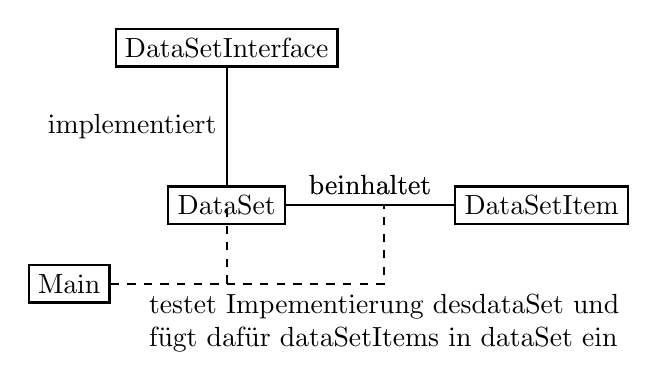
\begin{tikzpicture}[thick]
  \tikzset{
  op/.style={
    rectangle,
    draw=black
  }
}
\node[op] at (2,4)
  (datasetinterface) {DataSetInterface};
\node[op] at (2,2)
  (dataset) {DataSet};
\node[op] at (0,1)
  (Main) {Main};
\node[op] at (6,2)
  (datasetitem) {DataSetItem};

  \path
  (datasetinterface) edge node[left] {implementiert} (dataset);

  \path
  (dataset) edge node[above] {beinhaltet} (datasetitem);

   \path
  (dataset) edge node[above] {beinhaltet} (datasetitem);

    \draw[dashed] (Main) -- (2,1) -- (2,2) -- (dataset);
    \draw[dashed] (Main) -- (4,1)node[below, align=justify] {testet Impementierung desdataSet und\\ fügt dafür dataSetItems in dataSet ein} -- (4,2) -- (datasetitem);
  
\end{tikzpicture}
\end{center}

\subsection{Einleitung}
Ein Datensatz besteht aus mehreren Daten, ein einzelnes Datum wird durch ein Objekt der Klasse "DataSetItem" repräsentiert.
Jedes Datum hat einen Namen (Zeichenkette), eine ID (Zahl) und bel. Inhalt.\\
Nun sollen mehrere Daten, Objekte vom Typ "DataSetItem", in einem Datensatz zusammengefasst werden.
Sie haben sich schon auf eine Schnittstelle und die benötigen Operationen, die ein Datensatz unterstützen muss, geeinigt.
Es gibt eine Klasse "DataSetInterface", die die Schnittstelle definiert und Operationen jedes Datensatzes angibt.
Bisher fehlt aber noch die Implementierung eines Datensatzes mit allen Operationen.\\
\\
Implementieren Sie eine Klasse "DataSet" als eine Unterklasse von "DataSetInterface".\\
\\
\subsection{Aufbau}
Es gibt drei Dateien, "dataset.py", "main.py" und "implementation.py"$^*$.
In der "dataset.py" befinden sich die Klassen "DataSetInterface" und "DataSetItem",
in der Datei "implementation.py" muss die Klasse "DataSet" implementiert werden.
Die Datei "main.py" nutzt die Klassen "DataSet" und "DataSetItem" aus den jeweiligen Dateien und testet die Schnittstelle und Operationen von "DataSetInterface".\\
\\
\subsection{Methoden}
Bei der Klasse "DataSet" sind insbesondere folgenden Methoden zu implementieren, die genaue Spezifikation finden Sie in der "dataset.py":\\
    \begin{itemize}
        \item \bf setitem(self, name, id\_content)\normalfont\\
  Hinzufügen eines Datums, mit Name, ID und Inhalt
  \item \bf iadd(self, item))\normalfont\\
  Hinzufügen eines "DataSetItem"
  \item \bf delitem(self, name)\normalfont\\
  Löschen eines Datums auf Basis des Namens. Das heißt auch, dass der Name eines Datums ein eindeutiger Schlüssel ist und jeder Name nur einmal pro Datensatz vorkommen kann.
  \item \bf contains(self, name) \normalfont\\
  Prüfung ob ein Datum mit diesem Namen im Datensatz vorhanden ist.
  \item \bf getitem(self, name)\normalfont\\
  Abrufen des Datzns über seinem Namen 
  \item \bf and(self, dataset)\normalfont\\
  Schnittmenge zweier Datensätze bestimmen und als einen neuen Datensatz zurückgeben-
  \item \bf or(self, dataset)\normalfont\\
  Vereinigung zweier Datensätze bestimmen und als einen neuen Datensatz zurückgeben.
  \item \bf iter(self)\normalfont\\
  Iteration über alle Daten des Datensatzes(es ist möglich eine Sortierung für die Reihenfolge der Iteration anzugeben)
  \item \bf filterediterate(self, filter)\normalfont\\
  gefilterte Iteration über einen Datensatz, dabei dient eine Lambda Funktion mit den Parametern Name und ID für jedes Datum als Filter.
  \item \bf len(self)\normalfont\\
  Anzahl der Daten in einem Datensatz abrufen.\\
    \end{itemize}
  


\section{Abgabe}
\raggedright
Programmieren Sie die Klasse "DataSet" in der Datei "implementation.py" zur Lösung der oben beschrieben Aufgabe im VPL.
Sie können auch direkt auf Ihrem Computer programmieren, dazu finden Sie alle drei benötigten Dateien zum Download im Moodle.\\

Das VPL nutzt den gleichen Code, wobei die "main.py" um weitere Testfälle und Überprüfungen erweitert wurde.
Die Überprüfungen dienen dazu sicherzustellen, dass Sie die richtigen Klassen nutzen.\\

Dateien befinden sich im Ordner "/code/" dieses Git-Repositories.

\end{document}